% ============================================================
% ANEXO A: DETALLE DE LAS ARQUITECTURAS DE APRENDIZAJE PROFUNDO
% ============================================================

\chapter{Detalle de las Arquitecturas de Aprendizaje Profundo}
\label{appendix:arquitecturas}

En este anexo se describen con mayor profundidad las especificaciones
de diseño de las cuatro arquitecturas de redes neuronales evaluadas en este proyecto.

\section{ResNet 1D}
La red convolucional residual (ResNet 1D)\cite{he2015deepresiduallearningimage} implementa la arquitectura base para la extracción de rasgos morfológicos de los canales de ECG. 
La característica distintiva de ResNet es la adición de conexiones de atajo (\textit{skip connections})\cite{rajpurkar2017cardiologistlevelarrhythmiadetectionconvolutional}, que suman la entrada de un bloque residual a su salida:
\begin{equation}
\mathbf{y} = \mathcal{F}(\mathbf{x}, \{W_i\}) + W_s \mathbf{x}
\end{equation}
donde $\mathbf{x}$ e $\mathbf{y}$ son los vectores de entrada y salida, respectivamente, $\mathcal{F}$ representa la función de mapeo residual a aprender, y $W_s$ es una proyección lineal utilizada únicamente cuando es necesario ajustar las dimensiones de los canales.

El flujo detallado de la señal a través de la arquitectura y la concatenación de las características de variabilidad del ritmo cardíaco (HRV) se representan en la figura~\ref{fig:resnet}.

\begin{figure}[htbp]
  \centering
  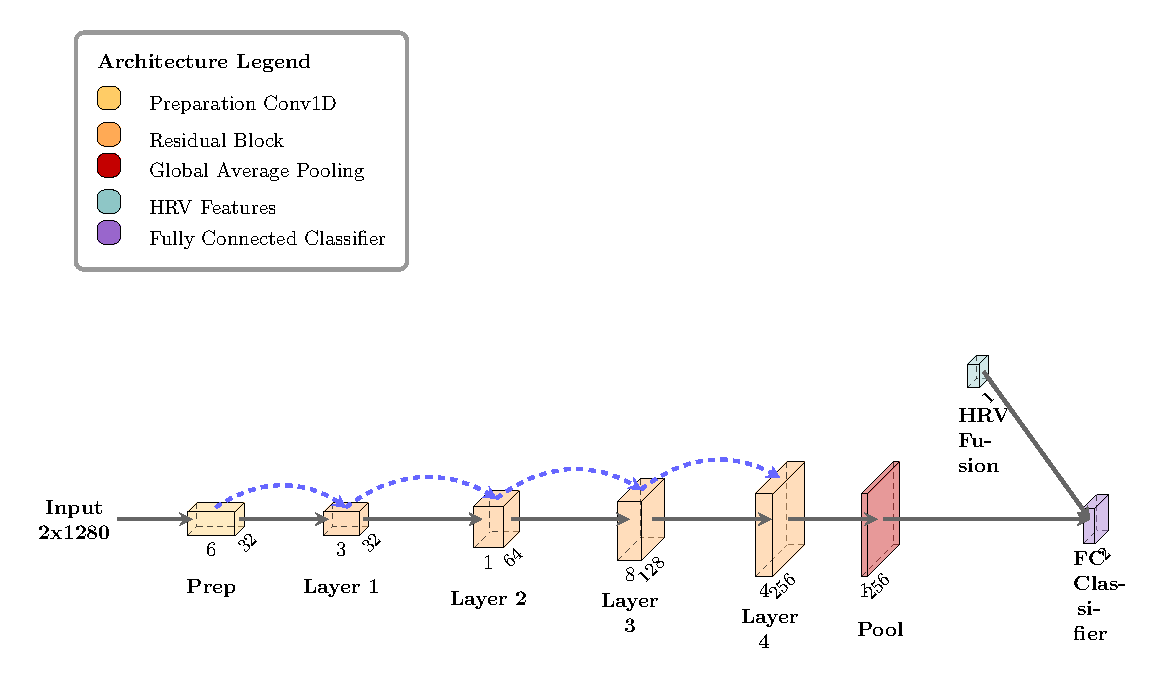
\includegraphics[width=0.9\textwidth]{img/resnet.pdf}
  \caption{Arquitectura base ResNet 1D. La red procesa la entrada reduciendo progresivamente la dimensión temporal mediante bloques residuales, integrando finalmente las características HRV antes del clasificador \textit{fully connected}.}
  \label{fig:resnet}
\end{figure}

\section{SEResNet 1D}
La arquitectura SEResNet 1D se basa en la incorporación de módulos \textit{Squeeze-and-Excitation}
(SE) en los bloques residuales convencionales. Esta adición tiene como objetivo recalibrar adaptativamente
las respuestas de los canales, modelando explícitamente las interdependencias entre ellos para mejorar
el rendimiento de la red.\cite{senet1d}

El módulo SE, detallado en la figura~\ref{fig:squeeze_and_excitation_block}, consta de dos pasos principales:

\begin{enumerate}
  \item \textbf{Squeeze (Compresión):} Se realiza un promedio global a lo largo de la dimensión temporal $L$ para resumir la información del canal $c$, produciendo un vector de características globales:
  \begin{equation}
    z_c = \frac{1}{L} \sum_{i=1}^{L} u_c(i)
  \end{equation}
  \item \textbf{Excitation (Excitación):} Se calcula una escala de pesos no lineal basada en las interdependencias de los canales mediante un cuello de botella con dos capas densas:
  \begin{equation}
    \mathbf{s} = \sigma(W_2 \cdot \text{ReLU}(W_1 \cdot \mathbf{z}))
  \end{equation}
  donde $\sigma$ es la función sigmoide, $W_1 \in \mathbb{R}^{\frac{C}{r} \times C}$ y $W_2 \in \mathbb{R}^{C \times \frac{C}{r}}$, siendo $r$ el factor de reducción.
\end{enumerate}

El esquema correspondiente al módulo SE se muestra en la figura~\ref{fig:squeeze_and_excitation_block}.

\begin{figure}[htbp]
  \centering
  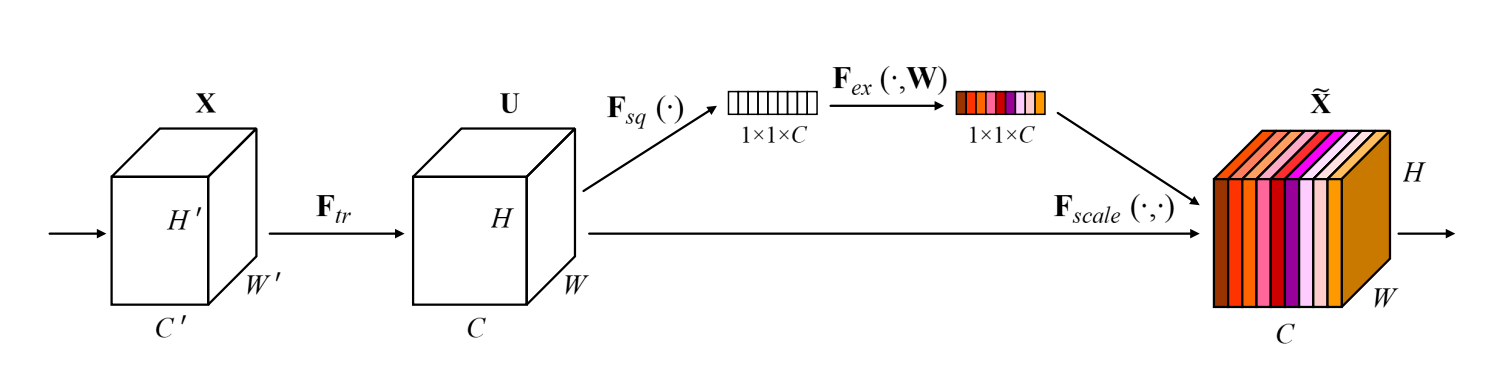
\includegraphics[width=0.9\textwidth]{img/squeeze-and-excitation-block} % Solo el nombre del archivo, sin extensión
  \caption{Módulo Squeeze-and-Excitation. Tras cada bloque residual se incorpora este módulo que
  recalibra adaptativamente los pesos de los canales. Obtenida del paper original \cite{senet1d}}
  \label{fig:squeeze_and_excitation_block}
\end{figure}

El flujo secuencial se ilustra en la figura~\ref{fig:seresnet}.

\begin{figure}[htbp]
  \centering
  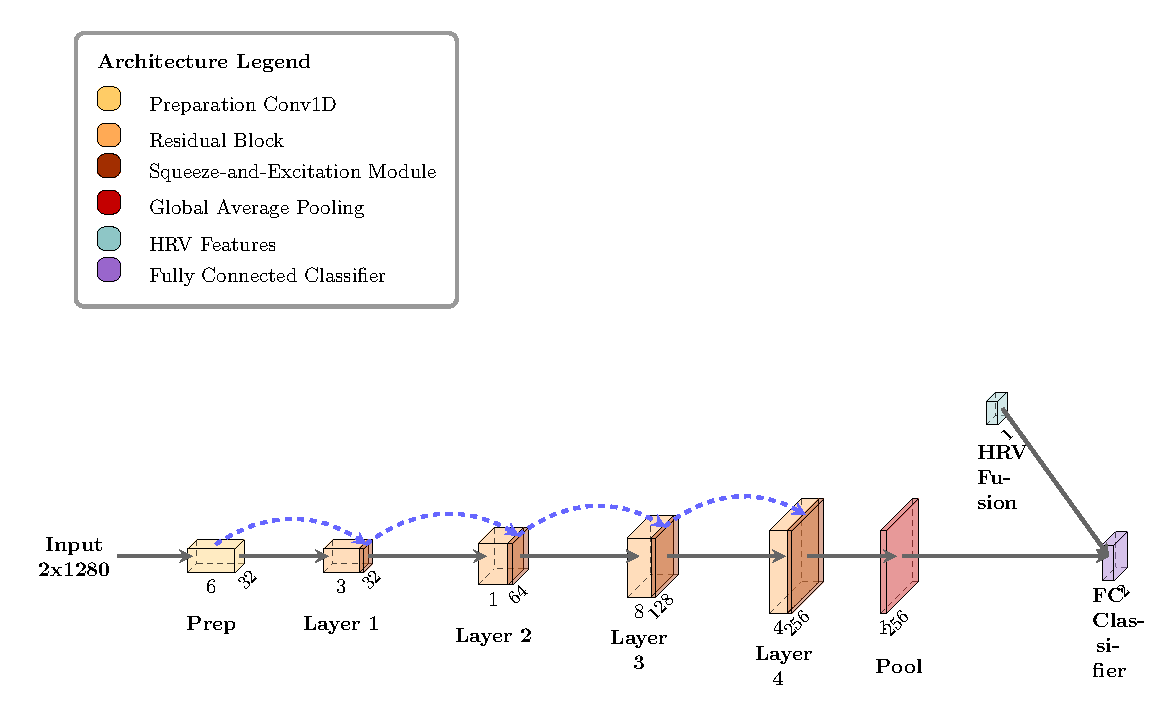
\includegraphics[width=0.9\textwidth]{img/seresnet.pdf}
  \caption{Arquitectura SEResNet 1D. Tras cada bloque residual se incorpora un módulo
  Squeeze-and-Excitation que recalibra adaptativamente los pesos de los canales de extracción de
  características.}
  \label{fig:seresnet}
\end{figure}

\section{CNN-Transformer Híbrido}
La arquitectura híbrida utiliza codificadores Transformer para capturar dependencias a largo plazo gracias al mecanismo de autoatención multifiltrada (\textit{Multi-Head Self-Attention}, MHSA).
Dada una matriz de proyección de consultas ($\mathbf{Q}$), claves ($\mathbf{K}$) y valores ($\mathbf{V}$), la atención de una sola cabeza se define como:
\begin{equation}
  \text{Attention}(\mathbf{Q}, \mathbf{K}, \mathbf{V}) = \text{softmax}\left(\frac{\mathbf{Q} \mathbf{K}^T}{\sqrt{d_k}}\right) \mathbf{V}
\end{equation}
donde $d_k$ es la dimensión de las claves. La autoatención concatena múltiples cabezas de atención
proyectadas linealmente para capturar diferentes relaciones de contexto simultáneamente. \cite{vaswani2023attentionneed}

El diagrama del codificador híbrido se muestra en la figura~\ref{fig:transformer}.

\begin{figure}[htbp]
  \centering
  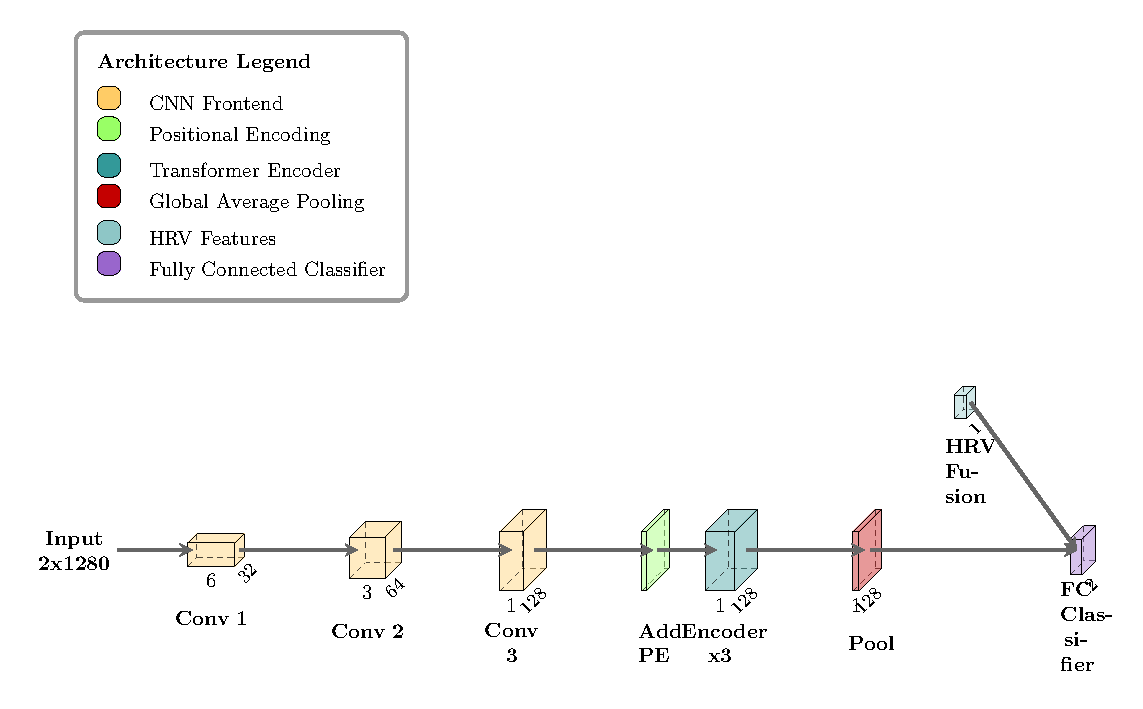
\includegraphics[width=0.9\textwidth]{img/transformer.pdf}
  \caption{Arquitectura híbrida CNN-Transformer. Se utiliza un \textit{frontend} convolucional para la extracción local y reducción de dimensionalidad, seguido de codificadores posicionales y un \textit{Transformer Encoder} para la atención global.}
  \label{fig:transformer}
\end{figure}

\section{Mamba 1D}
Mamba introduce los modelos de espacio de estados estructurados selectivos (\textit{Selective Structured State Space Models}, S4), los cuales permiten procesar secuencias con una complejidad temporal lineal respecto a la longitud de la entrada, manteniendo a la vez un mecanismo de atención selectivo basado en el contexto. 

En el dominio continuo, estos modelos mapean una señal unidimensional de entrada $x(t) \in \mathbb{R}$ a una representación latente e invisible $h(t) \in \mathbb{R}^N$ mediante una ecuación diferencial lineal de primer orden, para luego proyectarla hacia la salida $y(t) \in \mathbb{R}$:
\begin{equation}
  h'(t) = \mathbf{A} h(t) + \mathbf{B} x(t), \quad y(t) = \mathbf{C} h(t) + \mathbf{D} x(t)
\end{equation}

Para su implementación en datos discretos, estas ecuaciones se formulan mediante un paso de
discretización $\mathbf{\Delta}$. La principal innovación de Mamba radica en su mecanismo de selección,
haciendo que las matrices de transición $\mathbf{B}$ y $\mathbf{C}$, así como el propio parámetro
deescala $\mathbf{\Delta}$, sean funciones directas de la entrada $x_t$. Esto rompe la invarianza
en el tiempo de los SSM tradicionales y permite al sistema decidir activamente qué información
propagar o descartar a lo largo de la secuencia de manera dinámica. \cite{gu2024mambalineartimesequencemodeling}

La estructura interna del bloque Mamba y el flujo de los datos a través del módulo de selección se ilustran detalladamente en la figura~\ref{fig:mamba_block}.

\begin{figure}[htbp]
  \centering
  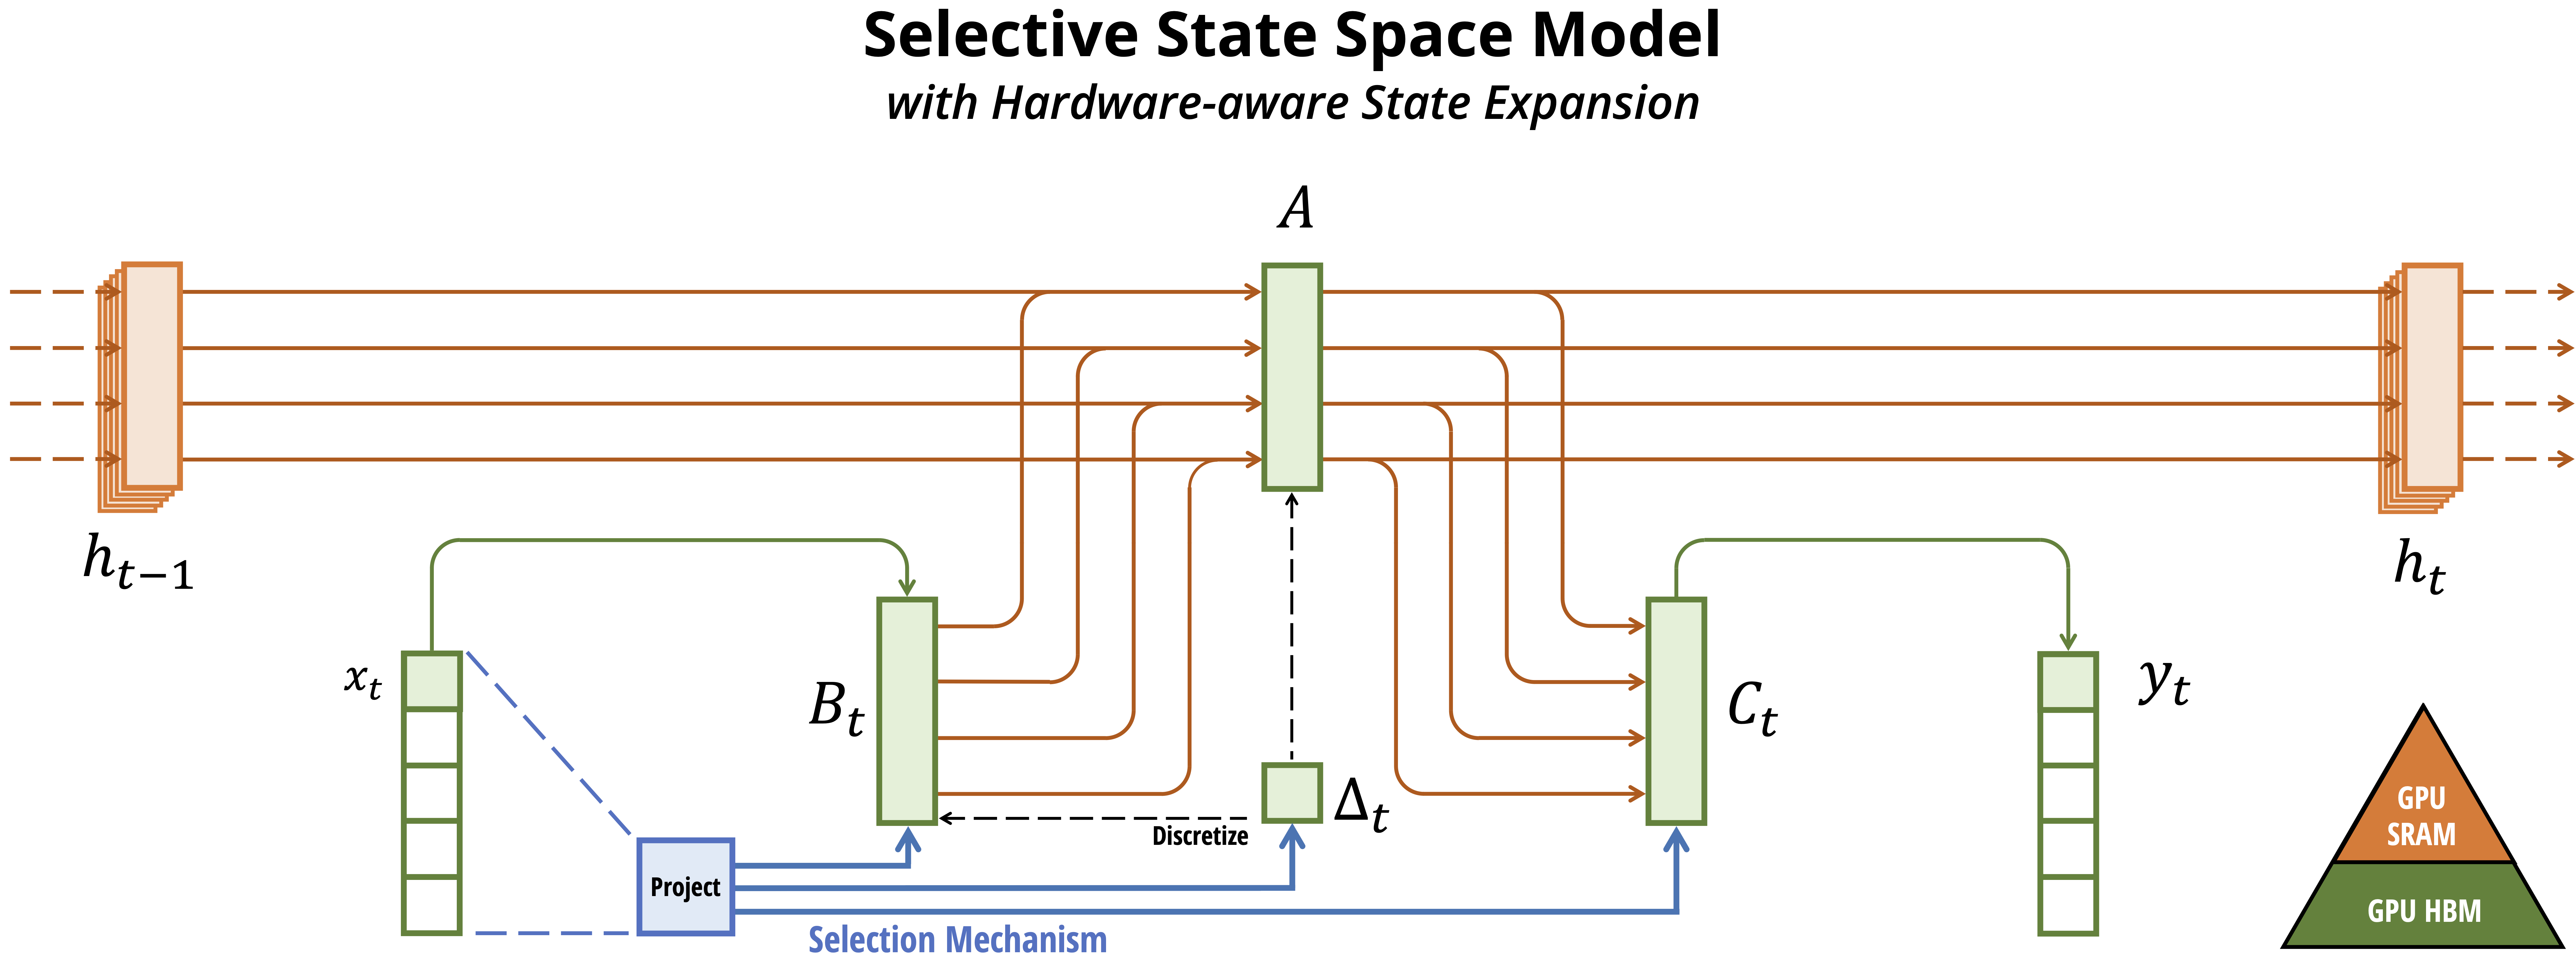
\includegraphics[width=0.9\textwidth]{img/mamba1} % Carga tu imagen del bloque interno
  \caption{Estructura interna del bloque Mamba. Se detalla el mecanismo del modelo de espacio de estados selectivo (SSM), donde los parámetros de discretización y transición se calculan de manera dinámica en función de la secuencia de entrada.}
  \label{fig:mamba_block}
\end{figure}

El flujo secuencial se ilustra en la figura~\ref{fig:mamba}.

\begin{figure}[htbp]
  \centering
  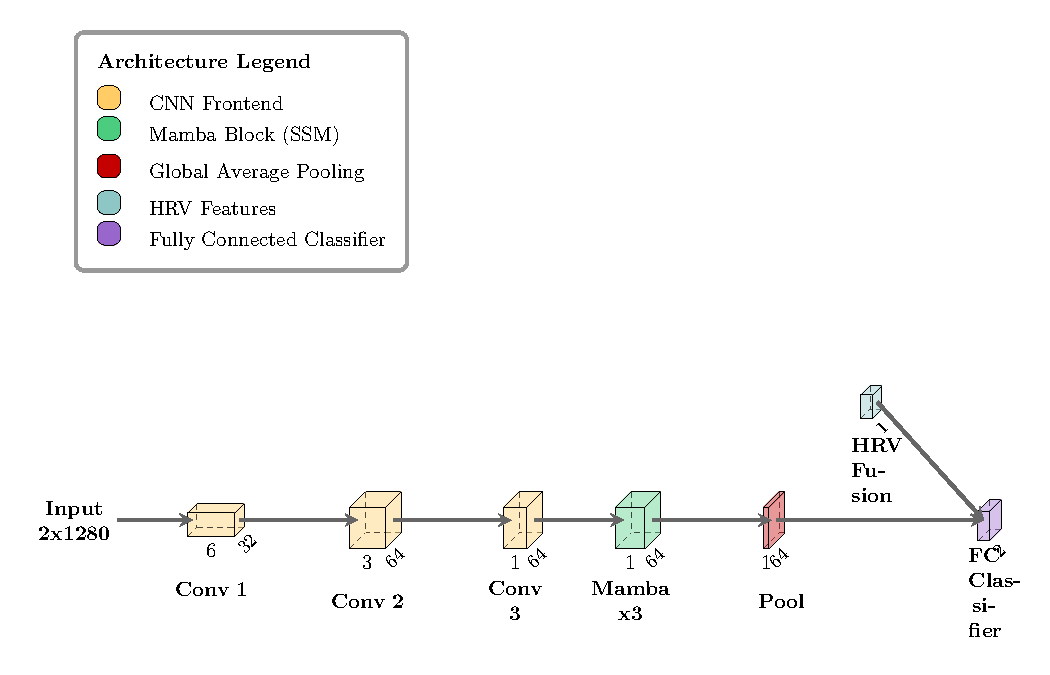
\includegraphics[width=0.9\textwidth]{img/mamba.pdf}
  \caption{Arquitectura híbrida CNN-Mamba. La secuencia latente generada por el \textit{frontend} convolucional es procesada de forma puramente secuencial mediante bloques SSM selectivos, prescindiendo de codificadores posicionales.}
  \label{fig:mamba}
\end{figure}